\documentclass{tufte-handout}

\title{On ultimate: dumps and retaining possession}
\author[James Reynolds]{James Reynolds}

%\date{28 March 2010} % without \date command, current date is supplied

%\geometry{showframe} % display margins for debugging page layout

\usepackage{graphicx} % allow embedded images
  \setkeys{Gin}{width=\linewidth,totalheight=\textheight,keepaspectratio}
  \graphicspath{{graphics/}} % set of paths to search for images
\usepackage{amsmath}  % extended mathematics
\usepackage{booktabs} % book-quality tables
\usepackage{units}    % non-stacked fractions and better unit spacing
\usepackage{multicol} % multiple column layout facilities
\usepackage{lipsum}   % filler text
\usepackage{fancyvrb} % extended verbatim environments
  \fvset{fontsize=\normalsize}% default font size for fancy-verbatim environments

% Standardize command font styles and environments
\newcommand{\doccmd}[1]{\texttt{\textbackslash#1}}% command name -- adds backslash automatically
\newcommand{\docopt}[1]{\ensuremath{\langle}\textrm{\textit{#1}}\ensuremath{\rangle}}% optional command argument
\newcommand{\docarg}[1]{\textrm{\textit{#1}}}% (required) command argument
\newcommand{\docenv}[1]{\textsf{#1}}% environment name
\newcommand{\docpkg}[1]{\texttt{#1}}% package name
\newcommand{\doccls}[1]{\texttt{#1}}% document class name
\newcommand{\docclsopt}[1]{\texttt{#1}}% document class option name
\newenvironment{docspec}{\begin{quote}\noindent}{\end{quote}}% command specification environment

\begin{document}

\maketitle% this prints the handout title, author, and date



%\printclassoptions


\begin{marginfigure}
\begin{equation}
A - C = 1 - B - D
\end{equation}
\end{marginfigure}
\begin{marginfigure}
\begin{equation}
A - C = B - D
\end{equation}
\end{marginfigure}

Defence wins games, 
offence loses them. 
This is because,
in ultimate,
the difference
in the number 
times possession
is lost 
(i.e. a turnover)
by each team
is related to 
the difference in 
the scores\footnote{
Let A 
be the score of 
the team with the
highest score,
and  B be the 
score of the 
other team; 
and let 
C and D
be the number
times possession
is lost 
by the team
with the highest score
and the other team, 
again respectively. 
Then, 
during the first half, 
at the end 
of a point when 
A + B is odd
or even, 
respectively, 
equations 1 
or 2 
apply.}\footnote{
Yes, 
it gets more complicated 
during the second half,
based on 
which team 
pulled first 
and which 
team scored 
the last point 
before half.  
Let's not 
get into that here.}. 
A team 
that (somehow)
never loses 
possession across
an entire game 
will defeat 
a team 
that loses possession 
only once or twice\footnote{
Again, 
there are edge cases, 
such as if 
no one can score 
upwind at all.}.


 
Hence, 
being able 
to retain possession 
is important\footnote{
More important than getting 
a big layout block on 
defence? Possibly, 
because at that point 
the job 
is only half done - 
your team still 
needs to convert 
the block into a goal!},
especially on 
points when 
your team 
receives 
the pull. 
A 'dump' throw,
or 'dumping it' 
back to one of the handlers, 
usually refers 
to a short 
throw, 
often backwards,
made to 
reset the stall count 
and retain possession 
of the disc. 
Being able 
to throw a dump 
is therefore a 
key skill 
for almost any
ultimate player. 
If you're a handler 
being able to 
set up for 
and then receive a dump 
is vital too\footnote{
With the rare exception of 
if you are on the defence team 
and the team's strategy is 
to score 
as soon as possible 
after getting a turnover 
and/or to accept 
higher risks
(e.g. run and gun, 
Huck and D,  
etc.).}.

This document is  
a two-pager about 
throwing or 
receiving a dump pass\footnote{
This
is part of a series, 
available at
\url{https://github.com/James-Reynolds/Ultimate-strategy-and-tactics}.}. 
It first discusses 
what a dump is 
and why it is important. 
Positioning for the dump 
is discussed, 
followed by how to 
engage with 'the dump'
and complete a dump pass. 
Finally, using 
dumps to generate 
offensive opportunities 
is discussed. 

There are 
many approaches 
and thoughts 
about ultimate 
strategy 
and tactics. 
Many
may disagree 
with what is 
written here. 
These are just 
my thoughts. 
Please feel free to 
fork or send pull requests.

\section{What is a dump and why is it important?}\label{sec:what_is_a_dump}
A backwards pass?  
A short pass?  
A pass 
to a handler?
It might be 
one 
or all 
of these, 
but typically 
a dump is about 
reseting the stall count, 
retaining possession, 
and/or improving the position
of the disc.  
Being able 
to complete 
dump throws 
is important because 
this impacts, 
and to an extent dictates, 
whether your team can 
play low-risk, high-completion 
offense. 
With an effective dump-set 
your team can retain possession
and wait for  
good opportunities.  
Without a reliable dump-set, 
you'll likely 
need to play higher-risk 
offence\footnote{
Huck-and-zone anyone? 
Not that there is anything 
wrong with huck-and-zone 
if it is working. 
Just that it 
will not 
work against teams
who don't turn the disc over much.}.  

Unfortunately, it's time for some more maths. 
The probability 
of losing possession
is a function of 
the number of passes made 
and the completion rate of 
each of those passes.
For example,  
if it takes 5 throws
to score and 
each has a 85\% chance 
of being completed
the overall chance 
of scoring is only 44\%
\begin{marginfigure}
\begin{equation} 0.85^5 = 0.44 \end{equation}
\end{marginfigure} 
In comparison
a 50-50 huck
to the endzone
straight off the pull 
isn't looking too bad.
%Of course, 
%if your team scores 
%you actually do 
%'lose' possession 
%of the disc, 
%in that your 
%team then 
%has to pull 
%the disc 
%to your opposition; 
%but your score 
%goes up 
%so that is good.
Reality is more complex, 
with different players 
on your team 
having different 
completion rates 
for different throws 
and situations. 
Then there are the 
\smallcaps{second-order factors},  
were in someone who could play a
low-risk, high-completion 
style of ultimate 
is instead taking riskier options 
because the average 
completion rate is 
ow enough that 
they might as well
take some high-risk
shots to score quickly, 
as there is likely to be 
a turnover soon anyway.
But, in general, 
if the average completion rate 
of your entire team goes up, 
it will make sense 
for everyone 
to take less risky options\footnote{
Again, returning to the one high-risk  
versus five lower-risk throws example, 
if the completion rate goes up 
to 95\%, we are now looking at: 
\begin{equation} 0.95^5 = 0.77 \end{equation}
...and suddenly that 50-50\% huck 
isn't looking too good anymore.}, 
which may further 
increase the completion rate
and chance of scoring
instead of 
(eventually)
losing possesion. 
Another way of looking at this 
is: (1) ultimate
is usually stacked towards 
the offence\footnote{
Unless the weather is 
excessively 
windy.} 
because (1a) it is non-contact 
and (1b) there is 
typically 
somewhere
to throw the disc to 
such that a defender 
can't get to it without running 
through the receive; 
and (2) all defences 
will eventually 
break down 
as it is impossible to 
cover everything 
for ever. 
Hence, 
(3) if your team 
can just hold onto
possession 
long enough
a low-risk
opportunity to 
advance the disc 
and/or score a goal 
is likely to 
become 
available. 

\section{Against zone defenses}
\subsection{Positioning}
\label{sec:zone_positioning}

\subsection{Engaging and completing}
\label{sec:zone_engaging}

\subsection{Gaining an advantage from dumping}
\label{sec:zone_advantage}


\section{Against person-match}
\subsection{Positioning}
\label{sec:person-match_positioning}

\subsection{Engaging and completing}
\label{sec:person-match_engaging}

\subsection{Gaining an advantage from dumping}
\label{sec:person-match_advantage}





\subsection{No one expects the dump to cut deep}





\begin{marginfigure}%
  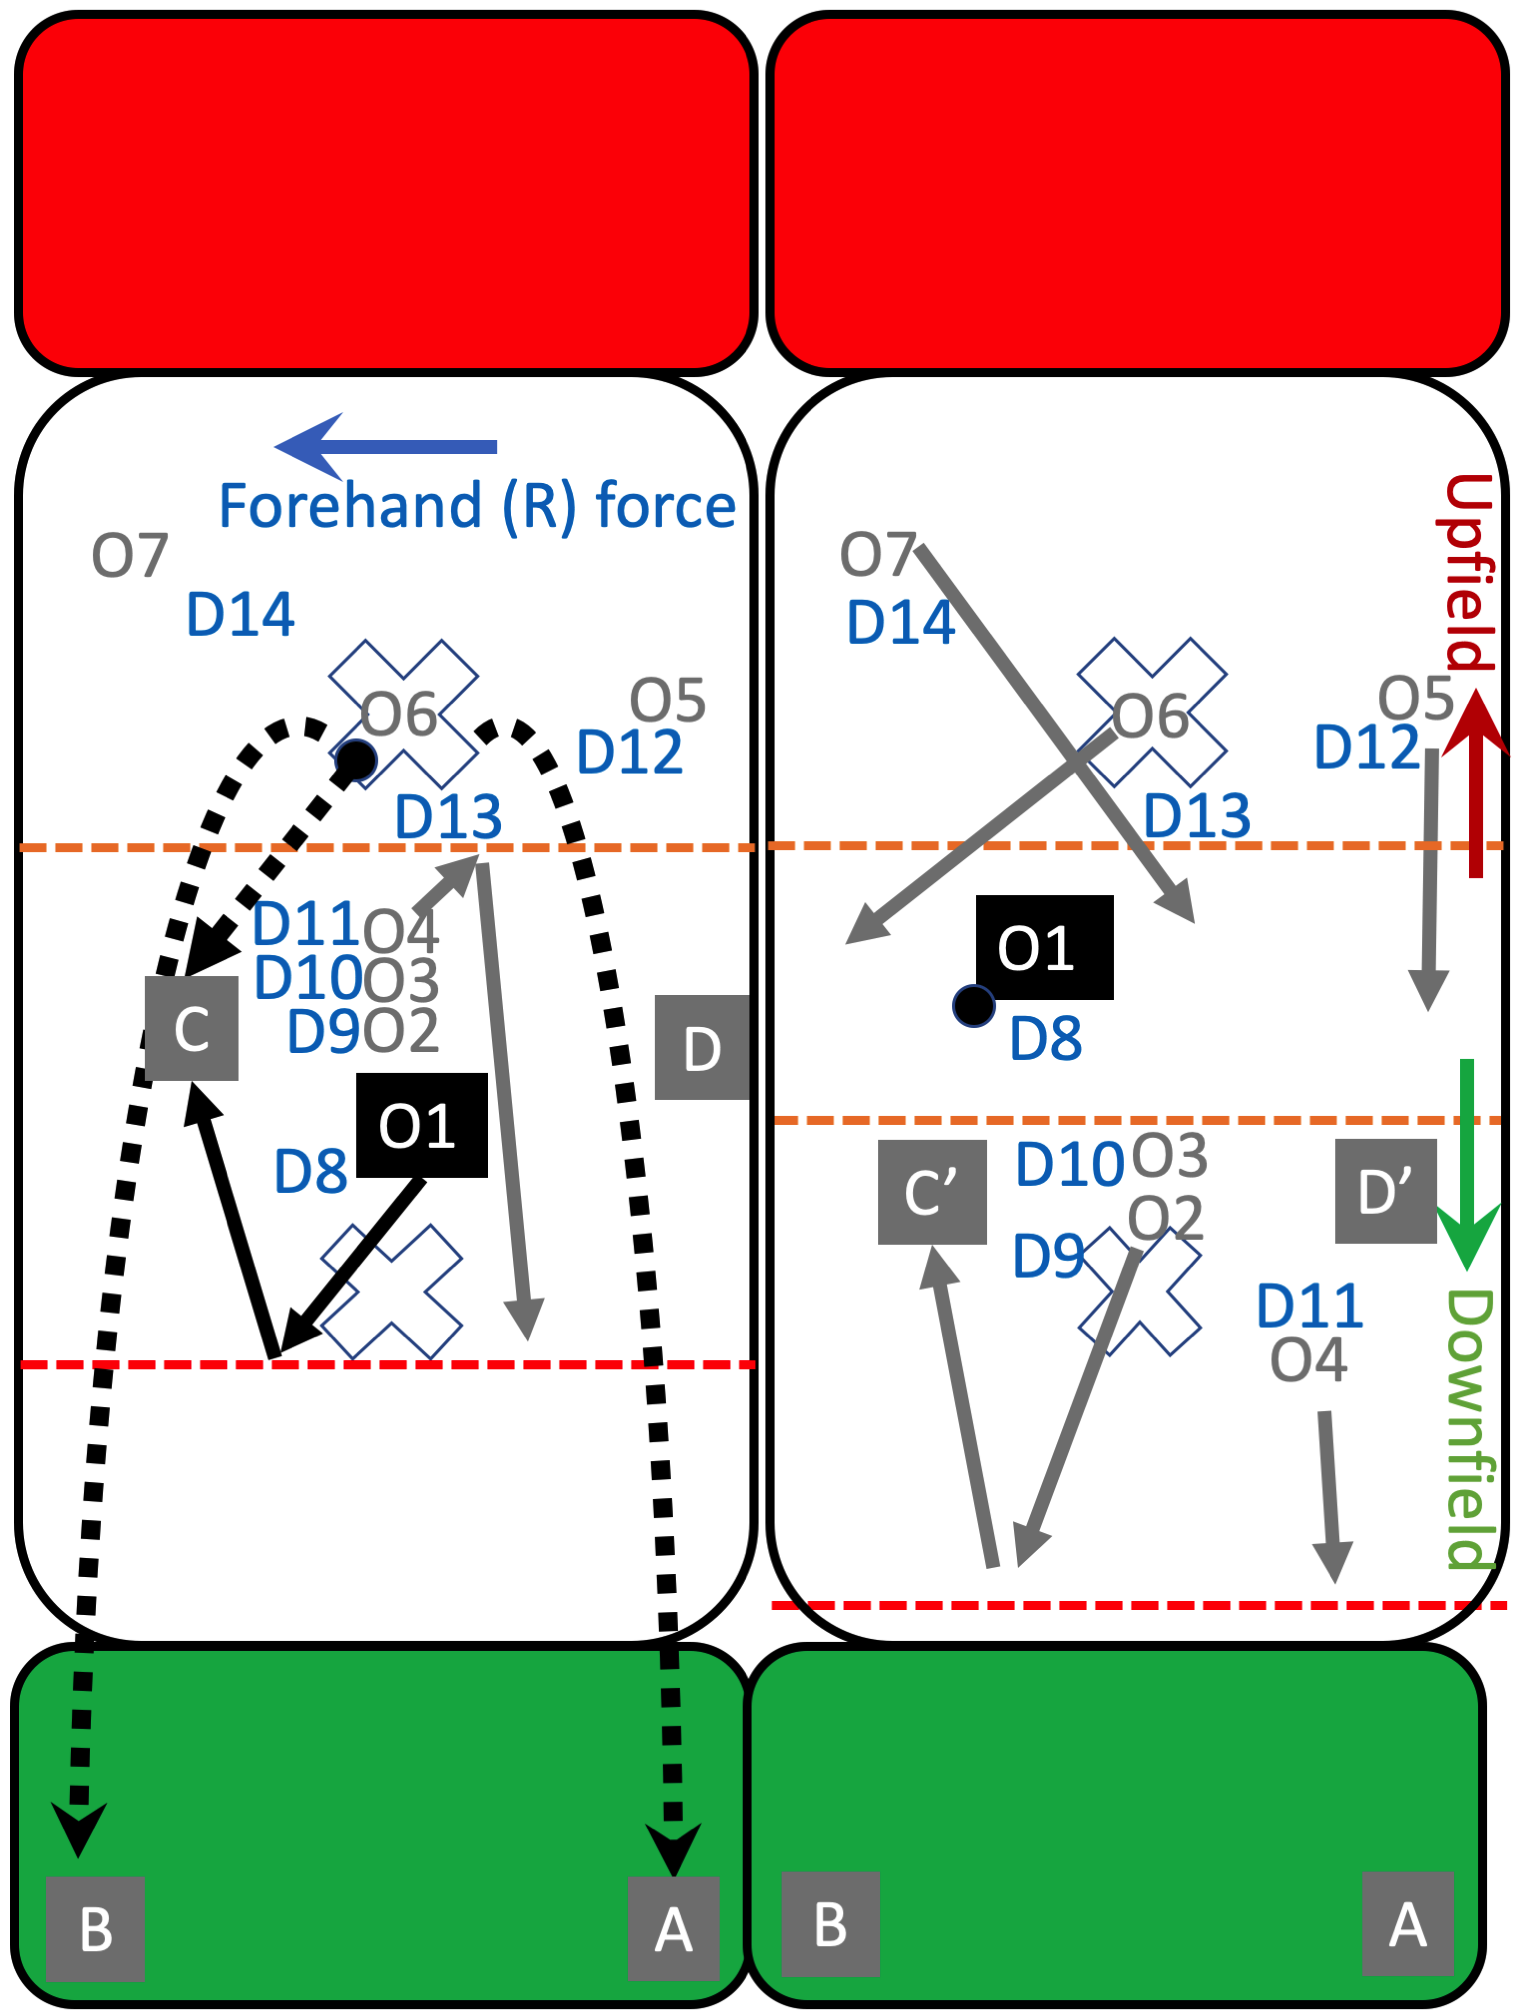
\includegraphics[width=\linewidth]{O1-vertical}
  \caption{Vertical stack: 
  starting position (left),
  and development (right)}
  \label{fig:O1-vertical}
\end{marginfigure}


\end{document}
